\documentclass[11pt,a4paper]{article}
\usepackage[T1]{fontenc}
\usepackage[utf8]{inputenc}
\usepackage{lmodern}
\usepackage[margin=20mm,headheight=15pt,headsep=7mm,footskip=10mm]{geometry}
\usepackage{microtype,amsmath,amssymb,graphicx,booktabs,tabularx,array}
\usepackage{xcolor,enumitem,fancyhdr,caption,hyperref,titlesec}
\definecolor{navy}{HTML}{18344A}
\definecolor{teal}{HTML}{167D8D}
\definecolor{muted}{HTML}{52616D}
\hypersetup{colorlinks=true,urlcolor=teal,linkcolor=navy,pdftitle={Temperature trends in Geneva: my progress and findings},pdfauthor={Ernest Terjyan}}
\pagestyle{fancy}
\fancyhf{}
\fancyhead[L]{\small\sffamily\color{muted}GENEVA TEMPERATURE TRENDS}
\fancyhead[R]{\small\sffamily\color{muted}Progress / 15 September 2026}
\fancyfoot[L]{\small\sffamily Ernest Terjyan}
\fancyfoot[R]{\small\sffamily\thepage}
\renewcommand{\headrulewidth}{0.3pt}
\setlength{\parindent}{0pt}
\setlength{\parskip}{4pt}
\titlespacing*{\section}{0pt}{8pt}{7pt}
\titlespacing*{\subsection}{0pt}{10pt}{3pt}
\setlist[itemize]{leftmargin=*,itemsep=3pt,topsep=3pt}
\setlist[enumerate]{leftmargin=*,itemsep=3pt,topsep=3pt}
\captionsetup{font=small,labelfont={bf,color=navy},skip=5pt,hypcap=false}
\newcommand{\heading}[1]{\section*{\sffamily\color{navy}#1}}
\newcommand{\subheading}[1]{\subsection*{\sffamily\color{navy}#1}}
\newcommand{\degreeC}{\ensuremath{{}^{\circ}\mathrm{C}}}
\newcommand{\pending}{\ensuremath{\square}}
\newcommand{\done}{\ensuremath{\checkmark}}
\newcommand{\sourceplot}[2]{\includegraphics[page=#1,width=#2]{../Rplots.pdf}}
\begin{document}
\thispagestyle{plain}
{\sffamily\color{teal}\small COMPUTATIONAL METHODS IN ECONOMETRICS}\par
\vspace{3mm}
{\sffamily\bfseries\color{navy}\fontsize{29}{33}\selectfont Temperature trends\\in Geneva}\par
{\large My progress, findings and next steps}\par
{\color{muted}Ernest Terjyan\enspace /\enspace 15 September 2026}
\vspace{2mm}

I am investigating whether a simple linear trend adequately describes Geneva's annual mean temperature record, and how residual dependence, changing variance and possible structural change affect inference. This is my ongoing working record for the group, based on the current files in my assignment folder.

\begin{quote}
\color{navy}\textbf{My current result.} I estimate an upward trend of \textbf{0.0337\degreeC{} per decade}. I have produced the residual diagnostics and calculated \textbf{DW = 1.4147}. The Monte Carlo test and Breusch--Pagan test are still unfinished.
\end{quote}

\heading{1. My data and current scope}
\begin{minipage}[t]{0.48\textwidth}
\vspace{0pt}
I use Station 08: Geneva, Switzerland. The supplied metadata identifies NOAA NCEI's GHCN Monthly Temperature Version 4, QCF adjusted series, as the source. Each annual mean requires at least ten valid monthly observations [1].

\small
\begin{tabularx}{\linewidth}{@{}Xr@{}}
\toprule
Recorded observations & 226\\
Recorded period & 1753--2013\\
Missing calendar years & 35\\
Incomplete supplied rows & 0\\
Duplicate years & 0\\
Mean temperature & 9.5034\degreeC\\
Minimum (1851) & 7.6483\degreeC\\
Maximum (2011) & 11.7300\degreeC\\
\bottomrule
\end{tabularx}
\end{minipage}\hfill
\begin{minipage}[t]{0.48\textwidth}
\vspace{0pt}
\sourceplot{1}{\linewidth}
\captionof{figure}{My original temperature-series plot. The line connects available observations, including across gaps.}
\end{minipage}

\textbf{My main data caveat:} all years from \textbf{1981 to 2009} are absent. Other missing years are 1931, 1968, 1973--1975 and 1979. My complete-case filter removes no rows. The connecting line from 1980 to 2010 does not represent observed annual movements in the missing period.

\textbf{What I have saved:} data preparation, OLS estimates, six plots and observed DW. My script ends immediately after the DW calculation. I have not yet implemented formal Monte Carlo calibration, BP, a structural-break search, bootstrap inference or the Part III experiment.

\newpage
\heading{2. My linear trend model}
I model annual mean temperature as a deterministic straight-line mean plus an error:
\[
y_i=\beta_0+\beta_1x_i+\varepsilon_i,
\qquad x_i=\frac{\mathrm{Year}_i-1900}{10}.
\]
I use $i$ to distinguish the observation's position from its calendar year. My transformation makes 1900 equal to zero and a ten-year increase equal to one unit. I transform time, not temperature. Thus $\beta_0$ is the fitted mean temperature in 1900 and $\beta_1$ is the trend in degrees Celsius per decade.

\subheading{How I estimate it}
I use \texttt{lm(Temperature \textasciitilde{} t, data = dat)}. Ordinary least squares chooses the intercept and slope that minimize
\[
\operatorname{RSS}(\beta_0,\beta_1)=\sum_{i=1}^{226}(y_i-\beta_0-\beta_1x_i)^2.
\]
My fitted equation is
\[
\boxed{\widehat y_i=9.61663+0.0337093x_i.}
\]

\begin{minipage}[t]{0.45\textwidth}
\vspace{0pt}
\small
\begin{tabularx}{\linewidth}{@{}Xr@{}}
\toprule
Quantity & Estimate\\
\midrule
Intercept & 9.6166\degreeC\\
Slope per decade & 0.03371\degreeC\\
Slope per century & 0.3371\degreeC\\
$R^2$ & 0.1054\\
Adjusted $R^2$ & 0.1014\\
Residual standard error & 0.6596\degreeC\\
Residual degrees of freedom & 224\\
\bottomrule
\end{tabularx}
\normalsize

I read $R^2$ as the share of variation around the sample mean explained by the fitted line: approximately 10.5\%. My residual standard error measures the estimated scale of deviations around that line.
\end{minipage}\hfill
\begin{minipage}[t]{0.52\textwidth}
\vspace{0pt}
\sourceplot{2}{\linewidth}
\captionof{figure}{My temperatures and fitted linear trend. The fit uses all 226 supplied observations.}
\end{minipage}

\subheading{What I can say at this stage}
I find a positive average slope over the supplied record. The fitted line rises by about \textbf{0.8764\degreeC{}} across 1753--2013, a 260-year span. This is a model-implied change, not the observed endpoint difference. Substantial variation remains around the line, and the four observations in 2010--2013 are all above it.

My printed OLS summary includes a conventional slope $p$-value of about $6.09\times10^{-7}$. I do not use it as a final significance conclusion: the residual diagnostics question the usual inference assumptions, and Part I explicitly postpones trend-significance conclusions [2].

\newpage
\heading{3. Residual patterns and dependence}
I define a residual as observed minus fitted temperature:
\[
\widehat\varepsilon_i=y_i-\widehat y_i.
\]
A positive residual means a warmer observation than my model predicts. A negative residual means a cooler observation. I use the residual time plot to look for remaining patterns and the ACF to examine dependence across observations.

\begin{minipage}[t]{0.48\textwidth}
\vspace{0pt}\sourceplot{3}{\linewidth}
\captionof{figure}{My residuals over calendar time, with a zero reference line. Units are \degreeC.}
\end{minipage}\hfill
\begin{minipage}[t]{0.48\textwidth}
\vspace{0pt}\sourceplot{4}{\linewidth}
\captionof{figure}{My residual ACF. Lags refer to adjacent available observations.}
\end{minipage}

\subheading{What I see in these plots}
I see runs of residuals on the same side of zero, including a negative stretch around the 1830s--1850s and positive residuals at the sample end. I interpret these patterns as reasons to investigate serial dependence and the adequacy of the mean trend. The time plot alone cannot distinguish those explanations or establish a structural break.

The ACF measures the association between residuals and lagged residuals. The values underlying my plot are approximately \textbf{0.290 at lag 1}, \textbf{0.218 at lag 2} and \textbf{0.185 at lag 3}. They exceed its approximate upper reference band of 0.130. I regard the bands as pointwise graphical guides. Lag zero equals one by construction.

\subheading{The Durbin--Watson statistic I have calculated}
My function at the end of \texttt{main.R} computes
\[
d=\frac{\sum_{i=2}^{n}(\widehat\varepsilon_i-\widehat\varepsilon_{i-1})^2}
{\sum_{i=1}^{n}\widehat\varepsilon_i^2},
\qquad\boxed{d_{\mathrm{obs}}=1.4147.}
\]
If adjacent residuals tend to move together, the numerator becomes smaller. The rough relation $d\approx2(1-\widehat\rho_1)$ explains the agreement with my positive lag-one ACF. Values below two suggest positive dependence; values above two suggest negative dependence. These are interpretive guides, not critical values.

\textbf{My present conclusion is graphical and descriptive.} I have not calculated a Monte Carlo rejection region or $p$-value. Also, both \texttt{acf()} and \texttt{diff()} use observation order: they treat 1980 and 2010 as consecutive observations. I cannot consistently call this lag ``one calendar year.''

\newpage
\heading{4. Residual magnitude and distribution}
I use two further plots to examine changing residual magnitudes and the shape of the residual distribution. Neither is a formal test in my current script.

\begin{minipage}[t]{0.48\textwidth}
\vspace{0pt}\sourceplot{5}{\linewidth}
\captionof{figure}{My squared residuals with a LOESS smoother. Squared residuals have units of $(\degreeC)^2$.}
\end{minipage}\hfill
\begin{minipage}[t]{0.48\textwidth}
\vspace{0pt}\sourceplot{6}{\linewidth}
\captionof{figure}{My normal Q--Q plot, comparing ordered residuals with normal quantiles.}
\end{minipage}

\subheading{Squared residuals and LOESS}
I square residuals to examine the size of deviations without their signs. LOESS fits local regressions to show a smooth pattern in those magnitudes. My curve rises into the early nineteenth century, declines toward the early twentieth century, and increases near the sample end.

I see possible variation in residual magnitude, but I have not established heteroskedasticity. A wrong mean specification can also generate large squared residuals. The recent increase requires particular caution because there are only four observations after 1980, separated from the earlier data by a long gap. The smooth curve across that gap does not supply missing evidence.

\subheading{Normal Q--Q plot}
In a Q--Q plot, I compare ordered residuals with theoretical normal-distribution quantiles. An approximately straight pattern is consistent with an approximately normal distribution. Most of my points follow the reference line reasonably closely, with some departures in the tails.

I do not treat this appearance as proof of normality. It also tells me nothing conclusive about independence or constant variance. Normality is not needed simply to compute the OLS coefficients.

\subheading{My combined assessment so far}
\begin{itemize}
\item I have an upward fitted trend, but the line leaves substantial variation unexplained.
\item My strongest current diagnostic concern is positive residual dependence, reflected in the ACF and observed DW.
\item I see possible changes in residual magnitudes, but my BP test remains to be done.
\item I need to distinguish dependence in the errors from remaining structure in the mean, particularly before choosing a bootstrap procedure.
\item I have no estimated break date and no statistical evidence from a completed break test yet.
\end{itemize}

\newpage
\heading{5. The formal tests I still need to finish}
\subheading{Durbin--Watson Monte Carlo calibration}
I have implemented the observed statistic only. The handout requires a two-sided Monte Carlo test with \textbf{$B=9{,}999$} and \textbf{$\alpha=0.05$} [2]. My next implementation needs to:
\begin{enumerate}
\item State the null error model, including the distribution, independence and variance assumptions. For example, an iid Gaussian null is stronger than merely assuming no first-order correlation.
\item Keep my observed regression design fixed, simulate errors under that null, and generate a simulated sample.
\item Refit the trend in every replication and calculate DW from the fitted residuals. Using raw simulated errors would omit the effect of estimating the trend.
\item Obtain separate 2.5\% and 97.5\% critical values, $c_L$ and $c_U$. I will reject when $d_{\mathrm{obs}}<c_L$ or $d_{\mathrm{obs}}>c_U$, without assuming symmetry around two.
\item Report both critical values, the Monte Carlo $p$-value, my tail-count convention and the conclusion. My script already sets seed \texttt{20260914}, but no simulation currently uses it.
\end{enumerate}

For example, I can document an equal-tail rank convention using
\[
p_L=\frac{1+\#\{d_b\leq d_{\mathrm{obs}}\}}{B+1},\qquad
p_U=\frac{1+\#\{d_b\geq d_{\mathrm{obs}}\}}{B+1},\qquad
p_{\mathrm{MC}}=\min\{1,2\min(p_L,p_U)\}.
\]
These formulas describe planned work; I have no simulated numerical results yet.

\subheading{The Breusch--Pagan auxiliary regression}
I still need to test for a systematic linear relationship between residual variance and my time regressor:
\[
\widehat\varepsilon_i^2=\gamma_0+\gamma_1x_i+v_i,
\qquad H_0:\gamma_1=0\quad\text{versus}\quad H_1:\gamma_1\ne0.
\]
The handout specifies $BP=nR^2_{\mathrm{aux}}$, using the $R^2$ from this auxiliary regression, not from the temperature regression. I will compare it with an asymptotic $\chi^2_1$ distribution and report its upper-tail $p$-value. I have one nonconstant variance regressor, which explains the one degree of freedom.

A failure to reject would not exclude every nonlinear variance pattern. I also need to qualify the usual chi-squared calibration in light of my residual dependence. The LOESS figure is not a completed BP test.

\subheading{A point I need to clarify in Question 6}
The required DW procedure simulates a finite-sample null distribution, whereas the specified BP calculation uses a large-sample approximation. I should not claim BP is inherently impossible to simulate. With fixed regressors and a specified iid Gaussian error model, both statistics are invariant to the regression coefficients and a common error scale. Monte Carlo calibration of heteroskedasticity tests is possible under suitable distributional assumptions [3]. I need to clarify the intended distinction with the lecturer; homoskedasticity alone does not specify a full finite-sample distribution.

\newpage
\heading{6. My next steps and working record}
\subheading{My immediate priorities}
\begin{itemize}[label=\pending]
\item Resolve the calendar-time versus observation-index convention with my group and lecturer, and document the missing years in figures and dependence measures.
\item Complete the DW Monte Carlo test and BP auxiliary regression, record their assumptions and numerical outputs, and interpret them together with my plots.
\item Write my own overall assessment of the initial model, keeping estimates, graphical indications and formal testing conclusions distinct.
\end{itemize}

\subheading{What I have not started in Parts II and III}
\begin{itemize}[label=\pending]
\item \textbf{Structural change:} search a continuous broken-trend model over admissible break dates with 15\% trimming; report the RSS profile, best-fitting calendar break and observed RSS reduction.
\item \textbf{Bootstrap inference:} justify a primary procedure and a sensitivity procedure using the diagnostics; use at least 999 replications for the reported break tests; construct percentile and percentile-$t$ slope intervals while re-estimating the break.
\item \textbf{Simulation study:} include no-break and break scenarios and vary at least two additional scenario dimensions; compare at least three bootstrap procedures with at least 1,000 Monte Carlo replications per configuration and 499 bootstrap replications within each, unless constraints are documented.
\end{itemize}
I maintain the fuller, editable checklist in \texttt{TODO.md}. The report deadline is \textbf{2 October 2026, 18:00}; the presentation deadline is \textbf{6 October 2026, 18:00}. I need a main report of no more than 15 pages and a 10-minute group presentation [2].

\subheading{Reproducibility and provenance}
I verified the unchanged \texttt{main.R} in a clean R 4.6.1 session with ggplot2. All six rendered plots reproduced the saved \texttt{Rplots.pdf} exactly. I captured the run in \texttt{docs/current-output.txt}. The data summaries and ACF values in this note were checked directly against the same data and fitted model; I have not represented them as separately implemented tests.

I run \texttt{make analysis} from the repository root and rebuild this document with \texttt{make report}. My LaTeX source embeds the original plot PDF pages directly. The report text is a dated snapshot, so I must refresh its numbers and interpretation when I change the analysis. Default \texttt{source()} may skip display of bare ggplot expressions; my verified route is \texttt{Rscript --vanilla main.R}.

\textbf{Assistance.} I have used ChatGPT/Codex for initial code suggestions, debugging and drafting documentation. The handout limits AI use to debugging and writing clarity, which I need to account for before assessed submission. I remain responsible for understanding the code and for my submitted analysis.

\vspace{1mm}
{\small
\textbf{Sources}\par
[1] Supplied \texttt{Station08.csv} and \texttt{Station08\_metadata.pdf}. NOAA NCEI, GHCN Monthly Temperature Version 4. DOI: \href{https://doi.org/10.7289/V5XW4GTH}{10.7289/V5XW4GTH}.\par
[2] Marina Friedrich, \emph{Computational Methods in Econometrics: Investigating Temperature Trends}, 2026--2027. Supplied \texttt{CMEAssignment2026Handout.pdf}.\par
[3] Dufour, Khalaf, Bernard and Genest (2004), \emph{Simulation-based finite-sample tests for heteroskedasticity and ARCH effects}, Journal of Econometrics 122, 317--347. \href{https://jeanmariedufour.github.io/Dufour_Khalaf_Bernard_Genest_2004_JE_HeteroskedasticityTests.pdf}{Research paper}.
}
\end{document}
